\documentclass{standalone}
\usepackage{tikz}
\begin{document}
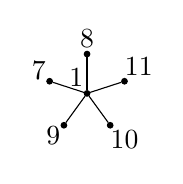
\begin{tikzpicture}[every node/.style={draw, circle, fill=black, minimum size=2pt, inner sep=0pt}]
\node[fill=black, label=above left:{$7$}] (G1N4) at (162:0.5) {};
\node[fill=black, label={[yshift=2pt]above left:{$1$}}] (G1N0) at (90:0) {};
\node[fill=black, label=above right:{$11$}] (G1N5) at (18:0.5) {};
\node[fill=black, label=above:{$8$}] (G1N1) at (90:0.5) {};
\node[fill=black, label=below left:{$9$}] (G1N3) at (234:0.5) {};
\node[fill=black, label=below right:{$10$}] (G1N2) at (306:0.5) {};
\draw (G1N0) -- (G1N1);
\draw (G1N0) -- (G1N2);
\draw (G1N0) -- (G1N3);
\draw (G1N0) -- (G1N4);
\draw (G1N0) -- (G1N5);
\end{tikzpicture}
\end{document}
